\documentclass[a4paper]{article}
\usepackage[utf8]{inputenc}
\usepackage[T1]{fontenc}
\usepackage{pdfpages}
\usepackage{lscape}
\usepackage[polish]{babel}
\usepackage{graphicx}
\usepackage[paper=portrait,pagesize]{typearea}

\title{Bazy danych 1}

\author{Leszek Błażewski, 241264 \\ \\Karol Noga, 241259}

\date{Semestr letni 2018/2019}

\begin{document}
\maketitle

\newpage

\section{Normalizacja bazy danych a redundancja}

Proces normalizacji bazy danych polega na doprowadzaniu bazy do postaci w której w bazie nie występuje redundancja. Redundancja jest zjawiskiem na ogół niepożądanym, lecz w specyficznych przypadkach jest konieczna w celu zapewnienia jakości danych usług (np. redundancja serwerów). Rozważając redundancję ze względu na dane występujące w bazie zauważyć możemy, że zjawisko to nie przynosi żadnych korzyści a jedynie przechowuje dane, które składowane są już w bazie tym samym zajmując miejsce, które wykorzystane mogłoby być na nowe informacje. Do redundancji dochodzić może gdy relacje pomiędzy obiektami nie zostały dokładnie przemyślane.

\section{Proces normalizacji}

Podczas pierwszej implementacji, nie zwróciliśmy uwagi na relacje zachodzące pomiędzy encją pracownika pływalni a jego czasem oraz dniami pracy. Pierwszym pomysłem było przechowywanie wszystkich danych dotyczących danego pracownika (włącznie z czasem pracy, dniami tygodnia gdy dana osoba pracuje oraz basenem do którego jest przydzielona) w tabeli $STAFF$. Takie rozwiązanie powodowało znaczne zwiększenie rozmiaru rekordów, co niekorzystnie wpłynęłoby na czas przeszukiwania danej tabeli. Problematyczne byłoby również przeszukiwanie tabeli w celu znalezienia pracowników pracujących w danych dniach, ponieważ każdy z rekordów odpowiadających danemu pracownikowi przechowywałby listę dni tygodnia przetrzymywaną w jednej kolumnie $WORKINGDAYS$, co kłóci się z pierwszą postacią normalną $(1NF)$.

\vspace{5mm}
Rozwiązaniem problemu jest wprowadzenie osobnej tabli $SCHEDULES$, która abstrahuje dane dotyczące czasu pracy oraz dni tygodnia od reszty informacji dotyczących pracownika. Tabela $SCHEDULES$ przechowuje klucz obcy do pracownika oraz do basenu, dzięki czemu znacznie redukujemy liczbę kolumn w tabeli i korzystamy z relacji klucz obcy -> główny. Rozwiązanie to też w prosty sposób pozwoliło uniknąć problemu przetrzymywania listy dni w jednej kolumnie, dzięki czemu pierwsza zasada postaci normalnej zostaje zachowana.

\vspace{5mm}
Poniżej zamieszczono diagram ER wygenerowany przy pomocy narzędzia Oracle SQL Developer Data Modeler.
\newpage
\KOMAoptions{paper=landscape,pagesize}
\recalctypearea
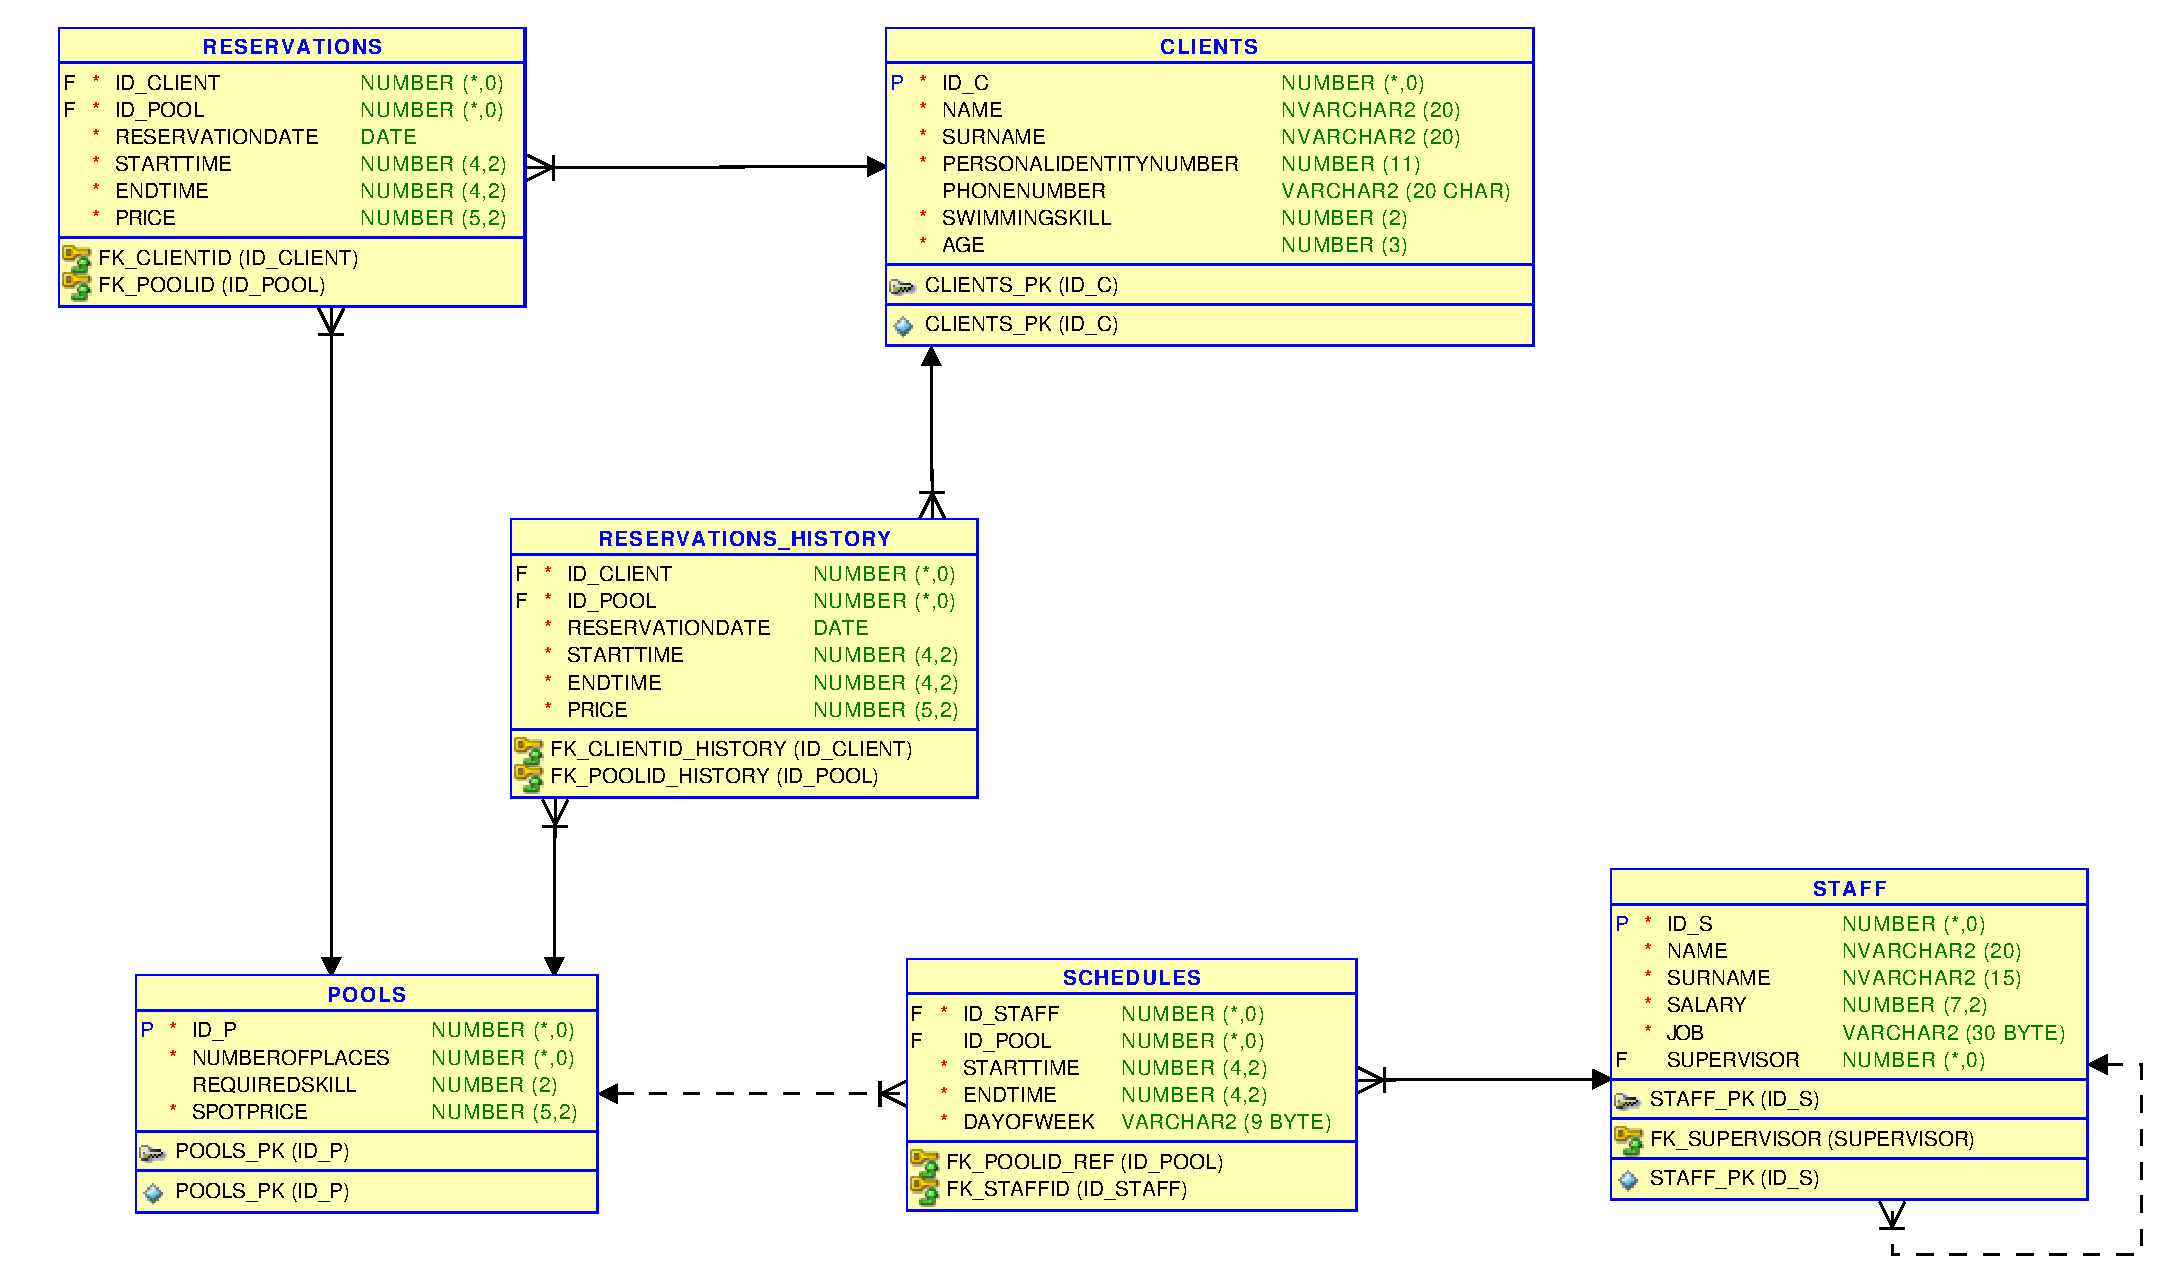
\includepdf[pages=-]{ERD_DIAGRAM.pdf}


\end{document}
